% 定义一些常用的颜色标注
\newcommand{\red}[1]{{\textcolor{red}{#1}}}%
% 定义一个数学公式
\newcommand{\argmin}{\mathop{\mathrm{argmin}}\limits}
\newcommand{\argmax}{\mathop{\mathrm{argmax}}\limits}
\chapter{公式、图表}
\section{公式}

方便快捷写入公式是\LaTeX 相对于Word编辑器最为主要的优势之一,特别是熟练掌握之后,在输入公式的时候具有非常大的提升效果。


\LaTeX 中的公式分为两类,包括有\red{行内公式}和\red{行间公式},例如这是一个行间公式$f(x)=\frac{1}{\sqrt{2\pi}\sigma}\exp\left(-\frac{(x-\mu)^{2}}{2\sigma^{2}}\right)$,下面举例几个行间公式

\begin{eqnarray}
    f(x)&=&\dfrac{1}{\sqrt{2\pi}\sigma}\exp\left(-\dfrac{(x-\mu)^{2}}{2\sigma^{2}}\right)    
\end{eqnarray}

例如,定义一个分段函数
\begin{eqnarray}
    f(x)&=&\begin{cases}
        -x^{3}+x+8&,x\leq{2}\\
        \dfrac{1}{2}x^{2}&,2<x\leq{10}\\
        x+10&,x>10
    \end{cases}
\end{eqnarray}

也可以定义一个多行的连等的等式,定义如下所示
\begin{eqnarray}
    \cos{2x}&=\cos^{2}x-\sin^{2}x\\
        &=2\cos^{2}x-1\\
        &=1-2\sin^{2}
\end{eqnarray}

可以将多个等式对齐写在同一个语句块当中,例如麦克斯韦方程组

积分形式:
\begin{equation}
    \begin{cases}
        \displaystyle\oint_{l}\mathbf{H}\cdot{d}\mathbf{l}&=\displaystyle\iint_\mathbf{S}J\cdot{d}\mathbf{S}+\displaystyle\iint_{S}\dfrac{\partial\mathbf{D}}{\partial{t}}\cdot{dS}\\
        \displaystyle\oint_{l}\mathbf{E}\cdot{d}\mathbf{l}&=-\displaystyle\iint_{S}\dfrac{\partial\mathbf{B}}{\partial{t}}\cdot{d}\mathbf{S}\\
        \displaystyle\oint_{S}\mathbf{B}\cdot{d}\mathbf{S}&=0\\
        \displaystyle\oint_{S}\mathbf{D}\cdot{d}\mathbf{S}&=\displaystyle\iiint_\mathbf{V}\rho{d}\mathbb{V}
    \end{cases}
\end{equation}

微分形式:
\begin{equation}
    \begin{cases}
        \nabla\times\mathbf{H}&=J+\dfrac{\partial\mathbf{D}}{\partial{t}}\\
        \nabla\times\mathbf{E}&=-\dfrac{\partial\mathbf{B}}{\partial{t}}\\
        \nabla\cdot\mathbf{B}&=0\\
        \nabla\cdot\mathbf{H}&=\rho\\
    \end{cases}
    \label{equ:diff-function}
\end{equation}

带有矩阵定义的公式:
\begin{equation}
    \mathbf{H} = -\mathbf\mu \cdot \mathbf{B} = -\gamma B_o \mathbf{S}_z = -\frac{\gamma B_o\hbar}{2} 
        \begin{bmatrix}
            1& \cdots &1\\ 
            \vdots & \ddots & \vdots \\
            1 & \cdots & 1 
        \end{bmatrix}.
    \label{equ:matrix}
\end{equation}

在求解凸优化问题的时候,问题研究最后求解归结为以下的方程形式:
\begin{equation}
    \argmin_{x_{j},j=1,\cdots,N}\sum\limits_{j=1}^{N}c_{j}x_{j}
\end{equation}
\begin{eqnarray}
    \text{s.t.}\begin{cases}
        \sum\limits_{j=1}^{N}a_{ij}x_{j}=b_{i},&i=1,\cdots,{m}\\
        x_{j}\geq{0},
    \end{cases}
\end{eqnarray}

在文章当中每一个公式的后面均可以添加一个label的标签,这样就可以应用公式了,例如\cref{equ:matrix}就是刚刚我们表达的矩阵表达式。

\section{画表}
\subsection{简单表格画法}
三线表画法:前面已经说明了三线表的画法,这里再次举例一个三线表,如表\ref{tab:heightweight}所示。

\begin{table}[!htp]
    \newcolumntype{L}{X}
    \newcolumntype{C}{>{\centering \arraybackslash}X}
    \newcolumntype{R}{>{\raggedright \arraybackslash}X}
    \centering
    \bicaption{某校学生身高体重样本}{Height and weight samples of students in a school}
    \label{tab:heightweight}
    \begin{tabularx}{0.9\textwidth}{CCCC}
       \toprule[1.5pt]
        序号&年龄&身高&体重\\
        \midrule[0.75pt]
        1&14&156&42\\
        2&16&158&45\\
        3&14&162&48\\
        4&15&163&50\\
        \midrule[0.75pt]
        %\cmidrule{2-4}
        平均&15&159.75&46.25\\
        \bottomrule[1.5pt]
    \end{tabularx}
\end{table}

表\ref{tab:some_products_datasets}所示是一个简单的双并排表的一个画法。
\begin{table}[htp!]
    \centering
    \bicaption{某行业产量与生产费用的数据}{Data of output and production cost of an industry}
    \label{tab:some_products_datasets}
    \newcolumntype{Y}{>{\centering\arraybackslash}X}
    \newcolumntype{Z}{!{\vline}@{\color{white}\vrule width \doublerulesep}!{\vrule}}%自定义列格式(双线)
    \begin{tabularx}{0.94\textwidth}{c|c|YZc|c|Y}
        \Xhline{0.9pt}
        企业编号&	产量(台)&生产费用(万元)&企业编号&产量(台)&生产费用(万元)\\
        \Xcline{1-3}{0.6pt}\Xcline{4-6}{0.6pt}
        1&	40&	130&7&	84&	165\\
        2&	42&	150&8&	100&	170\\
        3&	50&	155&9&	116&	167\\
        4&	55&	140&10&	125&	180\\
        5&	65&	150&11&	130&	175\\
        6&	78&	154&12&	140&	185\\
        \Xhline{0.72pt}
    \end{tabularx}
\end{table}

当然也可以画一个较为复杂的表,如表\ref{tab:model_dataset}所示

\begin{table}[hbpt]
    \centering
    \bicaption{一个数据表例子}{An example of a data table}
    \label{tab:model_dataset}
    \begin{tabular}{c|p{1cm}<{\centering}p{1cm}<{\centering}p{1cm}<{\centering}p{1cm}<{\centering}p{1cm}<{\centering}p{1cm}<{\centering}p{2cm}<{\centering}}
        \Xhline{2pt}
        Train & ND & YOS & LIB & YOS & LIB & ND & \multirow{2}{*}{Mean} \\
        \cmidrule(r){0-1}\cmidrule(lr){2-3}\cmidrule(lr){4-5}\cmidrule(lr){6-7}
        Test & \multicolumn{2}{c}{LIB} & \multicolumn{2}{c}{ND} & \multicolumn{2}{c}{YOS} &\\
        \Xcline{1-1}{0.4pt}
        \Xhline{1pt}
        
        SIFT [23] & \multicolumn{2}{c}{29.84} & \multicolumn{2}{c}{22.53} & \multicolumn{2}{c}{27.29} & 26.55\\
        TFeat [3] & 7.39 & 10.13 & 3.06 & 3.80 & 8.06 & 7.24 & 6.64 \\
        L2-Net [46] & 2.36 & 4.70 & 0.72 & 1.29 & 2.57 & 1.71 & 2.23 \\
        HardNet [26] & 1.49 & 2.51 & 0.53 & 0.78 & 1.96 & 1.84 & 1.51 \\
        DOAP [15] & 1.54 & 2.62 & 0.43 & 0.87 & 2.00 & 1.21 & 1.45 \\
        SOSNet [47] & 1.08 & 2.12 & 0.35 & 0.67 & 1.03 & \textbf{0.95} & 1.03 \\
        \textbf{HyNet} & \textbf{0.89} & \textbf{1.37} & \textbf{0.34} & \textbf{0.61} & \textbf{0.88} & 0.96 & \textbf{0.84} \\
        \Xhline{2pt}
    \end{tabular}
\end{table}

\newpage
\subsection{复杂表格画法}
如\cref{table:state-table-proposed-net}所示,这是一个跨页复杂表格的一个详细例子。
其中列举了表格的一些基本的画法,包括有跨页表格的画法,表格中的脚注的画法,表格中的多行合并的画法,表格中的多列合并的画法,表格中的多行多列合并的画。

\begin{ThreePartTable}
    \begin{TableNotes}
        \footnotesize
        \item [a] Euclidian Distance between output and target values
        \item [b] Fixed half-life values
        \item [c] Fixed regulatory parameters
        \item [d] Regulatory parameters
        \item [e] Half-maximal activation coefficients
        \item [f] Hill coefficient
    \end{TableNotes}
    \begin{longtable}{c l *{10}{c} c}
        % 表示的是第一次出现的表头信息
        \bicaption{应用基于Hill函数的方法得出的值:R1}{Derived Values from applying Hill-function based method: R1}\label{table:state-table-proposed-net}\\
        \toprule[1.5pt]
        Parameters & \multicolumn{10}{c}{Run}\\
        \cmidrule[1pt]{2-11}
        & 1 & 2 & 3 & 4 & 5 & 6 & 7 & 8 & 9 & 10\\
        \midrule[1pt]
        \endfirsthead

        % 下面是续表的表头信息。
        \bicaption{拟建网络的状态表(续)}{State Table for the proposed network (continued)}\\
        \toprule[1.5pt]
        Parameters & \multicolumn{10}{c}{Run}\\
        \cmidrule[1pt]{2-11}
        & 1 & 2 & 3 & 4 & 5 & 6 & 7 & 8 & 9 & 10\\
        \midrule[1.5pt]
        \endhead
    
        % 下面是续表的表尾信息。
        \bottomrule[1.5pt]
        \multicolumn{11}{r}{\small{注:其中$X\rightarrow{Y}$表示映射关系。接下页续表 $\rightarrow$}}\\
        \endfoot
    
        % 下面是最后表的表尾信息。
        \bottomrule[1.5pt]
        %告诉LaTeX在哪里插入“TableNotes”的内容
        \insertTableNotes  
        \endlastfoot
        % 下面是主体表所有的信息内容
    
        E.D.\tnote{a}  & 0.124 &  0.124 &  0.124 &  0.124 &  0.124 &  0.124 &  0.124 &  0.124 &  0.124 &  0.124 \\
        
        F.H.\tnote{b}  & 0.124 &  0.124 &  0.124 &  0.124 &  0.124 &  0.124 &  0.124 &  0.124 &  0.124 &  0.124 \\
        
        F.T.\tnote{c}  & 0.124 &  0.124 &  0.124 &  0.124 &  0.124 &  0.124 &  0.124 &  0.124 &  0.124 &  0.124 \\
        
        $T_{h \: \rightarrow \: o}$\tnote{d} & 0.124 &  0.124 &  0.124 &  0.124 &  0.124 &  0.124 &  0.124 &  0.124 &  0.124 &  0.124 \\
        
        $T_{g \: \rightarrow \: o}$ & 0.124 &  0.124 &  0.124 &  0.124 &  0.124 &  0.124 &  0.124 &  0.124 &  0.124 &  0.124 \\
        
        $T_{o \: \rightarrow \: h}$ & 0.124 &  0.124 &  0.124 &  0.124 &  0.124 &  0.124 &  0.124 &  0.124 &  0.124 &  0.124 \\
        
        $T_{g \: \rightarrow \: h}$ & 0.124 &  0.124 &  0.124 &  0.124 &  0.124 &  0.124 &  0.124 &  0.124 &  0.124 &  0.124 \\
        
        $T_{g \: \dashv \: c}$ & 0.124 &  0.124 &  0.124 &  0.124 &  0.124 &  0.124 &  0.124 &  0.124 &  0.124 &  0.124 \\
        
        $T_{g \: \dashv \: r}$ & 0.124 &  0.124 &  0.124 &  0.124 &  0.124 &  0.124 &  0.124 &  0.124 &  0.124 &  0.124 \\
        
        $K_{f \: \rightarrow \: o}$\tnote{e} & 0.124 &  0.124 &  0.124 &  0.124 &  0.124 &  0.124 &  0.124 &  0.124 &  0.124 &  0.124 \\
        
        $K_{h \: \rightarrow \: o}$ & 0.124 &  0.124 &  0.124 &  0.124 &  0.124 &  0.124 &  0.124 &  0.124 &  0.124 &  0.124 \\
        
        $K_{g \: \rightarrow \: o}$ & 0.124 &  0.124 &  0.124 &  0.124 &  0.124 &  0.124 &  0.124 &  0.124 &  0.124 &  0.124 \\
        
        $K_{f \: \rightarrow \: h}$ & 0.124 &  0.124 &  0.124 &  0.124 &  0.124 &  0.124 &  0.124 &  0.124 &  0.124 &  0.124 \\
        
        $K_{o \: \rightarrow \: h}$ & 0.124 &  0.124 &  0.124 &  0.124 &  0.124 &  0.124 &  0.124 &  0.124 &  0.124 &  0.124 \\
        
        $K_{g \: \rightarrow \: h}$ & 0.124 &  0.124 &  0.124 &  0.124 &  0.124 &  0.124 &  0.124 &  0.124 &  0.124 &  0.124 \\
        
        $K_{e \: \rightarrow \: g}$ & 0.124 &  0.124 &  0.124 &  0.124 &  0.124 &  0.124 &  0.124 &  0.124 &  0.124 &  0.124 \\
        
        $K_{f \: \rightarrow \: g}$ & 0.124 &  0.124 &  0.124 &  0.124 &  0.124 &  0.124 &  0.124 &  0.124 &  0.124 &  0.124 \\
        
        $K_{o \: \rightarrow \: g}$ & 0.124 &  0.124 &  0.124 &  0.124 &  0.124 &  0.124 &  0.124 &  0.124 &  0.124 &  0.124 \\
        
        $K_{h \: \rightarrow \: g}$ & 0.124 &  0.124 &  0.124 &  0.124 &  0.124 &  0.124 &  0.124 &  0.124 &  0.124 &  0.124 \\
        
        $K_{e \: \dashv \: c}$ & 0.124 &  0.124 &  0.124 &  0.124 &  0.124 &  0.124 &  0.124 &  0.124 &  0.124 &  0.124 \\
        
        $K_{e \: \dashv \: r}$ & 0.124 &  0.124 &  0.124 &  0.124 &  0.124 &  0.124 &  0.124 &  0.124 &  0.124 &  0.124 \\
        
        $K_{g \: \dashv \: c}$ & 0.124 &  0.124 &  0.124 &  0.124 &  0.124 &  0.124 &  0.124 &  0.124 &  0.124 &  0.124 \\
        
        $K_{g \: \dashv \: r}$ & 0.124 &  0.124 &  0.124 &  0.124 &  0.124 &  0.124 &  0.124 &  0.124 &  0.124 &  0.124 \\
        
        $K_{g \: \dashv \: o}$ & 0.124 &  0.124 &  0.124 &  0.124 &  0.124 &  0.124 &  0.124 &  0.124 &  0.124 &  0.124 \\
        
        $S_{c \: \rightarrow \: h}$\tnote{f} & 0.124 &  0.124 &  0.124 &  0.124 &  0.124 &  0.124 &  0.124 &  0.124 &  0.124 &  0.124 \\
        
        $S_{h \: \rightarrow \: o}$ & 0.124 &  0.124 &  0.124 &  0.124 &  0.124 &  0.124 &  0.124 &  0.124 &  0.124 &  0.124 \\
        
        $S_{g \: \rightarrow \: o}$ & 0.124 &  0.124 &  0.124 &  0.124 &  0.124 &  0.124 &  0.124 &  0.124 &  0.124 &  0.124 \\
        
        $S_{f \: \rightarrow \: h}$ & 0.124 &  0.124 &  0.124 &  0.124 &  0.124 &  0.124 &  0.124 &  0.124 &  0.124 &  0.124 \\
        
        $S_{o \: \rightarrow \: h}$ & 0.124 &  0.124 &  0.124 &  0.124 &  0.124 &  0.124 &  0.124 &  0.124 &  0.124 &  0.124 \\
        
        $S_{g \: \rightarrow \: h}$ & 0.124 &  0.124 &  0.124 &  0.124 &  0.124 &  0.124 &  0.124 &  0.124 &  0.124 &  0.124 \\
        
        $S_{e \: \rightarrow \: g}$ & 0.124 &  0.124 &  0.124 &  0.124 &  0.124 &  0.124 &  0.124 &  0.124 &  0.124 &  0.124 \\
        
        $S_{f \: \rightarrow \: g}$ & 0.124 &  0.124 &  0.124 &  0.124 &  0.124 &  0.124 &  0.124 &  0.124 &  0.124 &  0.124 \\
        
        $S_{o \: \rightarrow \: g}$ & 0.124 &  0.124 &  0.124 &  0.124 &  0.124 &  0.124 &  0.124 &  0.124 &  0.124 &  0.124 \\
        
        $S_{h \: \rightarrow \: g}$ & 0.124 &  0.124 &  0.124 &  0.124 &  0.124 &  0.124 &  0.124 &  0.124 &  0.124 &  0.124 \\
        
        $S_{e \: \dashv \: c}$ & 0.124 &  0.124 &  0.124 &  0.124 &  0.124 &  0.124 &  0.124 &  0.124 &  0.124 &  0.124 \\
        
        $S_{e \: \dashv \: r}$ & 0.124 &  0.124 &  0.124 &  0.124 &  0.124 &  0.124 &  0.124 &  0.124 &  0.124 &  0.124 \\
        
        $S_{g \: \dashv \: c}$ & 0.124 &  0.124 &  0.124 &  0.124 &  0.124 &  0.124 &  0.124 &  0.124 &  0.124 &  0.124 \\
        
        $S_{g \: \dashv \: r}$ & 0.124 &  0.124 &  0.124 &  0.124 &  0.124 &  0.124 &  0.124 &  0.124 &  0.124 &  0.124 \\
        
        $S_{g \: \dashv \: o}$ & 0.124 &  0.124 &  0.124 &  0.124 &  0.124 &  0.124 &  0.124 &  0.124 &  0.124 &  0.124 \\
    \end{longtable}
\end{ThreePartTable}


标准 LaTeX 提供有 array 和 tabular 两个制表环境,它们的完整格式如下:
\begin{enumerate}[label=(\arabic*)]
    \item \verb|\begin{array}[表格位置]{列样式}  \end{array}|

    \item \verb|\begin{tabular}[表格位置]{列样式}  \end{tabular}|
    
    \item \verb|\begin{tabular*}{表格总宽度}[表格位置]{列样式}  \end{tabular*}|
\end{enumerate}
这两个环境的选项和参数定义是相同的,不过 array 主要用于数组矩阵的排版,且只能用在数学环境中,如 equation 等。

扩展后的两个环境的列样式选项:

\begin{enumerate}[label=(\arabic*)]
    \item \verb|l|:列内容左对齐
    \item \verb|c|:列内容居中
    \item \verb|r|:列内容右对齐
    \item \verb|p{列宽}|:设置该列宽度,文本顶部对齐
    \item \verb|m{列宽}|:设置该列宽度,文本居中对齐
    \item \verb|b{列宽}|:设置该列宽度,文本底部对齐
    \item \verb|>{声明}|:声明可以是命令或插入列元素之前的文本
    \item \verb|<{声明}|:声明可以是命令或插入列元素之后的文本
    \item \verb|@{声明}|:该列每行插入声明中文本
    \item \verb|*{重复次数}{列样式}|:重复列样式
    \item \verb|!{文本}|:在文本前后插入 \verb|\arrayrulewidth|
    \item \verb|@{}|:取消列间的 \verb|\tabcolsep|
    \item \verb|@{|:在列前插入 \verb|\tabcolsep|
    \item \verb|@}|:在列后插入 \verb|\tabcolsep|
    \item \verb|||:列边或列之间插入竖线
\end{enumerate}

\section{画图}
本章节介绍图片插入方法,一共有三种插入图片的方法,我在下面详细介绍。
\subsection{普通插图方法}
如图\ref{fig:my_pic1}所示,在这里我们插入了一个图片。其中可以自定义缩放比例以及图片的高度等等信息。
\begin{figure}[hbpt]
    \centering
    \includegraphics[width=0.9\textwidth]{figures/test.jpg}
    \bicaption{这里插入了一个普通的相片}{An ordinary photo is inserted here}
    \label{fig:my_pic1}
\end{figure}
\subsection{多图插图方法}
多图插图方法主要是用到subfloat来进行插图处理。
\begin{figure}[htbp]
    \centering
    \subfloat[泰山]{
        \begin{minipage}[t]{0.48\linewidth}
            \centering
            \includegraphics[width=0.9\linewidth]{figures/taishan.jpeg}
        \end{minipage}
    }\vspace{-0.1cm}
    \subfloat[桂林山水]{
        \begin{minipage}[t]{0.48\linewidth}
            \centering
            \includegraphics[width=0.9\linewidth]{figures/guilin.jpeg}
        \end{minipage}
    }\vspace{-0.1cm}
    \subfloat[锡林郭勒盟草原]{
        \begin{minipage}[t]{0.48\linewidth}
            \centering
            \includegraphics[width=0.9\linewidth]{figures/xilinguole.jpeg}
        \end{minipage}
    }\vspace{-0.1cm}
    \subfloat[布达拉宫]{
        \begin{minipage}[t]{0.48\linewidth}
            \centering
            \includegraphics[width=0.9\linewidth]{figures/budalagong.jpeg}
        \end{minipage}
    }
    \centering
    \bicaption{示例的四张风景图片}{Four landscape pictures of the example}
\end{figure}

\subsection{latex自带的一些插图方法}

另外一种就是latex自带的一种画图方法,这里示例两种latex自带的画图方法。
\begin{enumerate}
    \item \textbf{复杂网络结构图}:如图\ref{fig:complex_fig}(a) 所示。
    \item \textbf{函数图像}:如图\ref{fig:complex_fig}(b),(c) 所示,详细参考\href{https://pgfplots.sourceforge.net/gallery.html},函数图像的画法使用到的是pgfplots库当中的元素画图。
\end{enumerate}

\begin{figure}
    \centering
    \subfloat[复杂网络结构图]{
        \begin{minipage}[t]{0.9\linewidth}
            \centering
            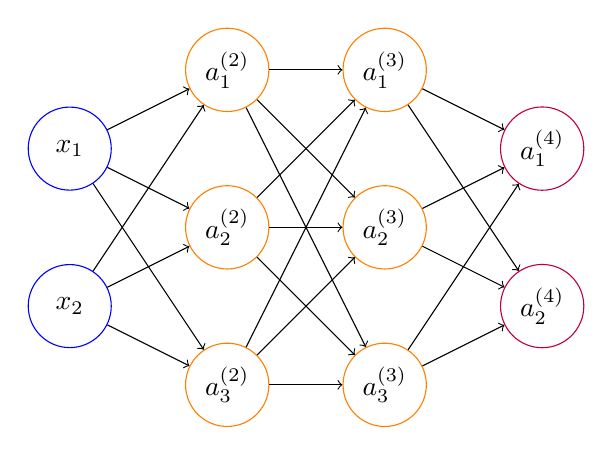
\begin{tikzpicture}
                \node[circle,
                    minimum width =30pt ,
                    minimum height =30pt ,draw=blue] (1) at(0,2){$x_1$};
                \node[circle,
                    minimum width =30pt ,
                    minimum height =30pt ,draw=blue] (2) at(0,0){$x_2$};
                \node[circle,
                    minimum width =30pt ,
                    minimum height =30pt ,draw=orange] (3) at(2,-1){$a_3^{(2)}$};
                \node[circle,
                    minimum width =30pt ,
                    minimum height =30pt ,draw=orange] (4) at(2,1){$a_2^{(2)}$};
                \node[circle,
                    minimum width =30pt ,
                    minimum height =30pt ,draw=orange] (5) at(2,3){$a_1^{(2)}$};
                \node[circle,
                    minimum width =30pt ,
                    minimum height =30pt ,draw=orange] (6) at(4,-1){$a_3^{(3)}$};
                \node[circle,
                    minimum width =30pt ,
                    minimum height =30pt ,draw=orange] (7) at(4,1){$a_2^{(3)}$};
                \node[circle,
                    minimum width =30pt ,
                    minimum height =30pt ,draw=orange] (8) at(4,3){$a_1^{(3)}$};
                \node[circle,
                    minimum width =30pt ,
                    minimum height =30pt ,draw=purple] (9) at(6,2){$a_1^{(4)}$};
                \node[circle,
                    minimum width =30pt ,
                    minimum height =30pt ,draw=purple] (10) at(6,0){$a_2^{(4)}$};
                \draw[->] (1) --(3);
                \draw[->] (1) --(4);
                \draw[->] (1) --(5);
                \draw[->] (2) --(3);
                \draw[->] (2) --(4);
                \draw[->] (2) --(5);
                \draw[->] (3) --(6);
                \draw[->] (3) --(7);
                \draw[->] (3) --(8);
                \draw[->] (4) --(6);
                \draw[->] (4) --(7);
                \draw[->] (4) --(8);
                \draw[->] (5) --(6);
                \draw[->] (5) --(7);
                \draw[->] (5) --(8);
                \draw[->] (6) --(9);
                \draw[->] (6) --(10);
                \draw[->] (7) --(9);
                \draw[->] (7) --(10);
                \draw[->] (8) --(9);
                \draw[->] (8) --(10);
            \end{tikzpicture}
        \end{minipage}
    }\vspace{-0.1cm}
    \subfloat[函数图像]{
        \begin{minipage}[t]{0.4\linewidth}
            \centering
            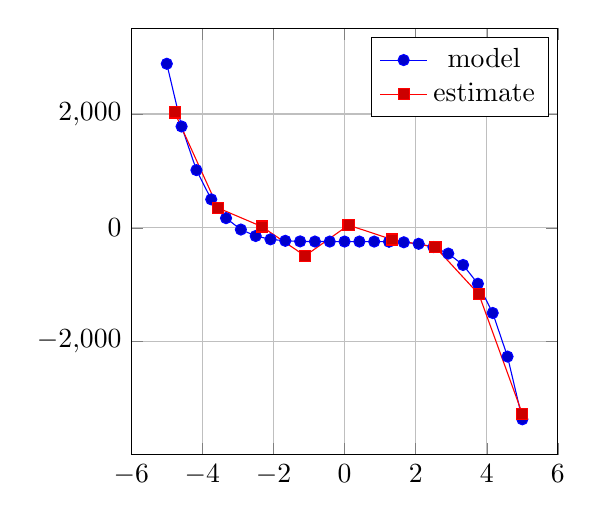
\begin{tikzpicture}
                \begin{axis}[
                    height=7cm,
                    width=7cm,
                    grid=major,
                ]
                    
                \addplot {-x^5 - 242};
                \addlegendentry{model}
            
                \addplot coordinates {
                    (-4.77778,2027.60977)
                    (-3.55556,347.84069)
                    (-2.33333,22.58953)
                    (-1.11111,-493.50066)
                    (0.11111,46.66082)
                    (1.33333,-205.56286)
                    (2.55556,-341.40638)
                    (3.77778,-1169.24780)
                    (5.00000,-3269.56775)
                };
                \addlegendentry{estimate}
                \end{axis}
            \end{tikzpicture}
        \end{minipage}
    }\vspace{-0.1cm}
    \quad
    \subfloat[统计图]{
        \begin{minipage}[t]{0.4\linewidth}
            \centering
            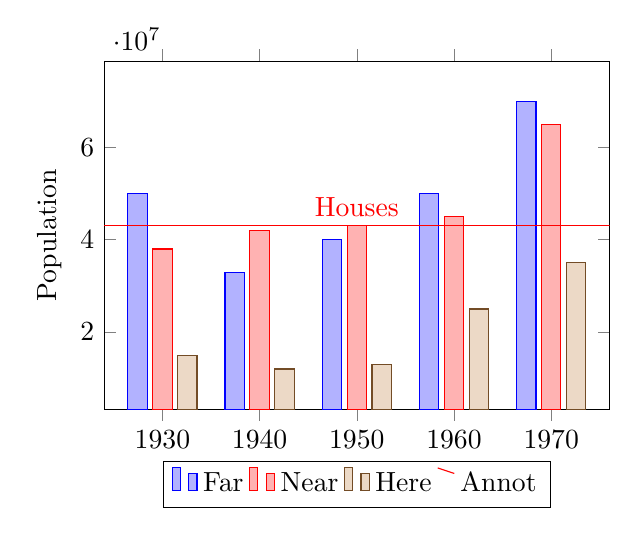
\begin{tikzpicture}
                \begin{axis}[
                    height=6cm,
                    width=8cm,
                    x tick label style={
                        /pgf/number format/1000 sep=},
                    ylabel=Population,
                    enlargelimits=0.15,
                    legend style={at={(0.5,-0.15)},
                        anchor=north,legend columns=-1},
                    ybar,
                    bar width=7pt,
                ]
                \addplot 
                    coordinates {(1930,50e6) (1940,33e6)
                         (1950,40e6) (1960,50e6) (1970,70e6)};
                
                \addplot 
                    coordinates {(1930,38e6) (1940,42e6) 
                        (1950,43e6) (1960,45e6) (1970,65e6)};
                
                \addplot 
                    coordinates {(1930,15e6) (1940,12e6) 
                        (1950,13e6) (1960,25e6) (1970,35e6)};
                
                \addplot[red,sharp plot,update limits=false] 
                    coordinates {(1910,4.3e7) (1990,4.3e7)} 
                    node[above] at (axis cs:1950,4.3e7) {Houses};
                
                \legend{Far,Near,Here,Annot}
                \end{axis}
            \end{tikzpicture}
        \end{minipage}
    }
    \bicaption{latex自带工具画图}{Drawing of latex built-in tools}
    \label{fig:complex_fig}
\end{figure}

\subsection{几个较为不错的画图例子}

使用pgfplots构建图,如\cref{fig:figure_ext1}所示。
这里给出了三个例子,分别是空间向量分布图,三维函数图像空间分布图,三角权重图。

\begin{figure}[htbp]
    \centering
    \subfloat[空间向量分布图]{
        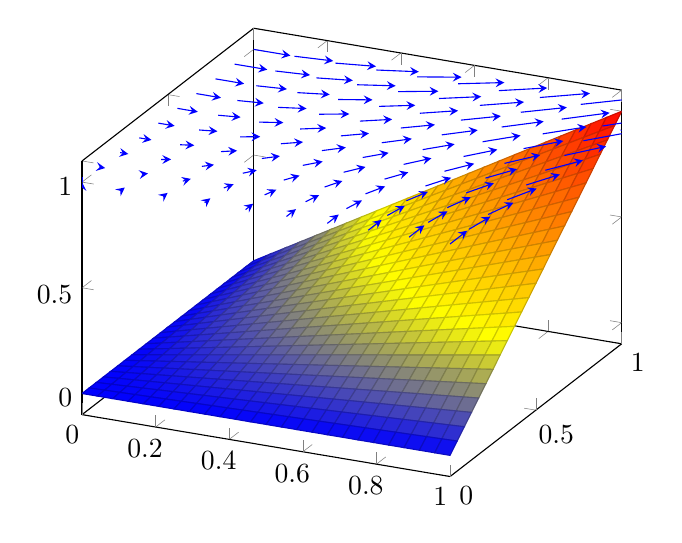
\begin{tikzpicture}
            \begin{axis}[
                domain=0:1,
                xmax=1,
                ymax=1,
            ]
            \addplot3[surf] {x*y};
            \addplot3[blue,/pgfplots/quiver,
                quiver/u=y,
                quiver/v=x,
                quiver/w=0,
                quiver/scale arrows=0.1,
                -stealth,samples=10] {1};
            \end{axis}
        \end{tikzpicture}
    }
    \subfloat[三维函数图像空间分布图]{
        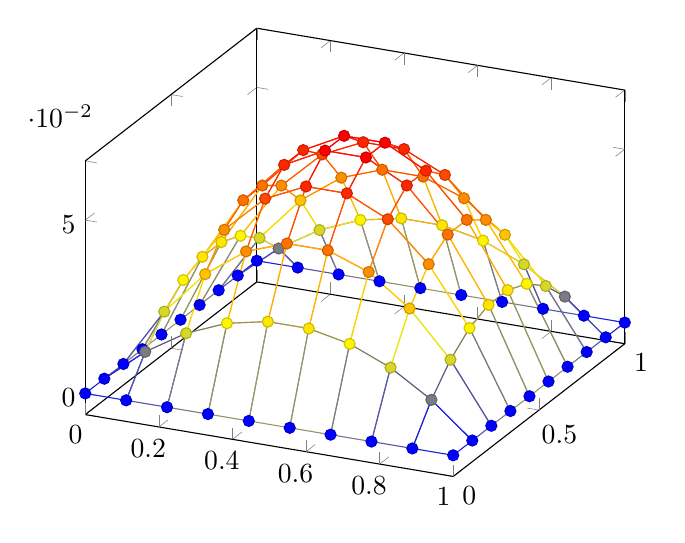
\begin{tikzpicture}
            \begin{axis}
            \addplot3+[mesh,scatter,samples=10,domain=0:1] 
                {x*(1-x)*y*(1-y)};
            \end{axis}
        \end{tikzpicture}
    }
    \quad
    \subfloat[三角权重图]{
        \begin{tikzpicture}
            \begin{ternaryaxis}[
                title=Want--be--Stainless Steel,
                xlabel=Weight Percent Chromium,
                ylabel=Weight Percent Iron,
                zlabel=Weight Percent Nickel,
                label style=sloped,
                area style,
            ]
                \addplot3 table[row sep=crcr] {
                A B C \\
                1 0 0 \\
                0.5 0.4 0.1 \\
                0.45 0.52 0.03 \\
                0.36 0.6 0.04 \\
                0.1 0.9 0 \\
                };
                \addlegendentry{Cr}
            
                \addplot3 table[row sep=crcr] {
                A B C \\
                1 0 0 \\
                0.5 0.4 0.1 \\
                0.28 0.35 0.37 \\
                0.4 0 0.6 \\
                };
                \addlegendentry{Cr+$\gamma$FeNi}
            
                \addplot3 table[row sep=crcr] {
                0.4 0 0.6 \\
                0.28 0.35 0.37 \\
                0.25 0.6 0.15 \\
                0.1 0.9 0 \\
                0 1 0 \\
                0 0 1 \\
                };
                \addlegendentry{$\gamma$FeNi}
            
                \addplot3 table[row sep=crcr] {
                0.1 0.9 0 \\
                0.36 0.6 0.04 \\
                0.25 0.6 0.15 \\
                };
                \addlegendentry{Cr+$\gamma$FeNi}
            
                \addplot3 table[row sep=crcr] {
                0.5 0.4 0.1 \\
                0.45 0.52 0.03 \\
                0.36 0.6 0.04 \\
                0.25 0.6 0.15 \\
                0.28 0.35 0.37 \\
                };
                \addlegendentry{$\sigma$+$\gamma$FeNi}
            
                \node[inner sep=0.5pt,circle,draw,fill=white,pin=-15:\footnotesize Stainless Steel] 
                  at (axis cs:0.18,0.74,0.08) {};
                
            \end{ternaryaxis}
        \end{tikzpicture}
    }
    \bicaption{几个较为不错的画图例子}{Several good examples of drawing}
    \label{fig:figure_ext1}
\end{figure}

\newpage
\subsection{神经网络图画法}
pgfplots 具有强大的功能,可以画出各种各样的图,可以画出较为不错的神经网结构图。
详细可以参考tikz网址\footnote{https://tikz.net/}以及pgfplots参考网址\footnote{https://tikz.dev/pgfplots/}\footnote{https://tikz.dev/}举个例子

\begin{figure}[hbpt]
    \centering
    % Command \empt{var1}{var2}
    \newcommand{\empt}[2]{$#1^{\langle #2 \rangle}$}
    \begin{tikzpicture}[
        % GLOBAL CFG
        font=\sf \scriptsize,
        >=LaTeX,
        % Styles
        cell/.style={% For the main box
            rectangle, 
            rounded corners=5mm, 
            draw,
            very thick,
            },
        operator/.style={%For operators like +  and  x
            circle,
            draw,
            inner sep=-0.5pt,
            minimum height =.2cm,
            },
        function/.style={%For functions
            ellipse,
            draw,
            inner sep=1pt
            },
        ct/.style={% For external inputs and outputs
            circle,
            draw,
            line width = .75pt,
            minimum width=1cm,
            inner sep=1pt,
            },
        gt/.style={% For internal inputs
            rectangle,
            draw,
            minimum width=4mm,
            minimum height=3mm,
            inner sep=1pt
            },
        mylabel/.style={% something new that I have learned
            font=\scriptsize\sffamily
            },
        ArrowC1/.style={% Arrows with rounded corners
            rounded corners=.25cm,
            thick,
            },
        ArrowC2/.style={% Arrows with big rounded corners
            rounded corners=.5cm,
            thick,
            },
        ]
    
        %Start drawing the thing...    
        % Draw the cell: 
        \node [cell, minimum height =4cm, minimum width=6cm] at (0,0){} ;
    
        % Draw inputs named ibox#
        \node [gt] (ibox1) at (-2,-0.75) {$\sigma$};
        \node [gt] (ibox2) at (-1.5,-0.75) {$\sigma$};
        \node [gt, minimum width=1cm] (ibox3) at (-0.5,-0.75) {Tanh};
        \node [gt] (ibox4) at (0.5,-0.75) {$\sigma$};
    
       % Draw opérators   named mux# , add# and func#
        \node [operator] (mux1) at (-2,1.5) {$\times$};
        \node [operator] (add1) at (-0.5,1.5) {+};
        \node [operator] (mux2) at (-0.5,0) {$\times$};
        \node [operator] (mux3) at (1.5,0) {$\times$};
        \node [function] (func1) at (1.5,0.75) {Tanh};
    
        % Draw External inputs? named as basis c,h,x
        \node[ct, label={[mylabel]Cell}] (c) at (-4,1.5) {\empt{c}{t-1}};
        \node[ct, label={[mylabel]Hidden}] (h) at (-4,-1.5) {\empt{h}{t-1}};
        \node[ct, label={[mylabel]left:Input}] (x) at (-2.5,-3) {\empt{x}{t}};
    
        % Draw External outputs? named as basis c2,h2,x2
        \node[ct, label={[mylabel]Label1}] (c2) at (4,1.5) {\empt{c}{t}};
        \node[ct, label={[mylabel]Label2}] (h2) at (4,-1.5) {\empt{h}{t}};
        \node[ct, label={[mylabel]left:Label3}] (x2) at (2.5,3) {\empt{h}{t}};
    
    % Start connecting all.
        %Intersections and displacements are used. 
        % Drawing arrows    
        \draw [ArrowC1] (c) -- (mux1) -- (add1) -- (c2);
    
        % Inputs
        \draw [ArrowC2] (h) -| (ibox4);
        \draw [ArrowC1] (h -| ibox1)++(-0.5,0) -| (ibox1); 
        \draw [ArrowC1] (h -| ibox2)++(-0.5,0) -| (ibox2);
        \draw [ArrowC1] (h -| ibox3)++(-0.5,0) -| (ibox3);
        \draw [ArrowC1] (x) -- (x |- h)-| (ibox3);
    
        % Internal
        \draw [->, ArrowC2] (ibox1) -- (mux1);
        \draw [->, ArrowC2] (ibox2) |- (mux2);
        \draw [->, ArrowC2] (ibox3) -- (mux2);
        \draw [->, ArrowC2] (ibox4) |- (mux3);
        \draw [->, ArrowC2] (mux2) -- (add1);
        \draw [->, ArrowC1] (add1 -| func1)++(-0.5,0) -| (func1);
        \draw [->, ArrowC2] (func1) -- (mux3);
    
        %Outputs
        \draw [-, ArrowC2] (mux3) |- (h2);
        \draw (c2 -| x2) ++(0,-0.1) coordinate (i1);
        \draw [-, ArrowC2] (h2 -| x2)++(-0.5,0) -| (i1);
        \draw [-, ArrowC2] (i1)++(0,0.2) -- (x2);
    
    \end{tikzpicture}
    \bicaption{LSTM 网络结构图}{LSTM network structure diagram}
\end{figure}


\input{texfigs/tensor.tex}

\input{texfigs/lenet5.tex}

\input{texfigs/gan.tex}

\input{texfigs/surface.tex}



